\chapter{Experimental Context}
\label{chap:context}

As discussed in \autoref{sec:gmsb}, the lack of coverage of the displaced dilepton signature leaves a sensitivity gap in \ac{LHC}-accessible \ac{SUSY}. All other searches for signatures that include displaced leptons also required a secondary vertex and are not sensitive to \slep production. The two $\ell$ from pair-produced \slep do not originate from the same decay so they are not connected by a vertex. Furthermore, since the $\tilde{G}$ is uncharged it leaves no track so there is no secondary vertex in the event.

The lifetime of the \slep is related to the \ac{SUSY} breaking scale (see \autoref{eq:lt}) which is not known, thus a suite of searches must be done to study the range of detector signatures corresponding to the range of possible lifetimes. This chapter will discuss the two previous searches for the displaced leptons signature, as well as the other searches that provide sensitivity to long lived \slep with different lifetimes. The different track signatures discussed in this chapter are shown in \autoref{fig:track-sigs}.

\begin{figure}[!h]
\centering
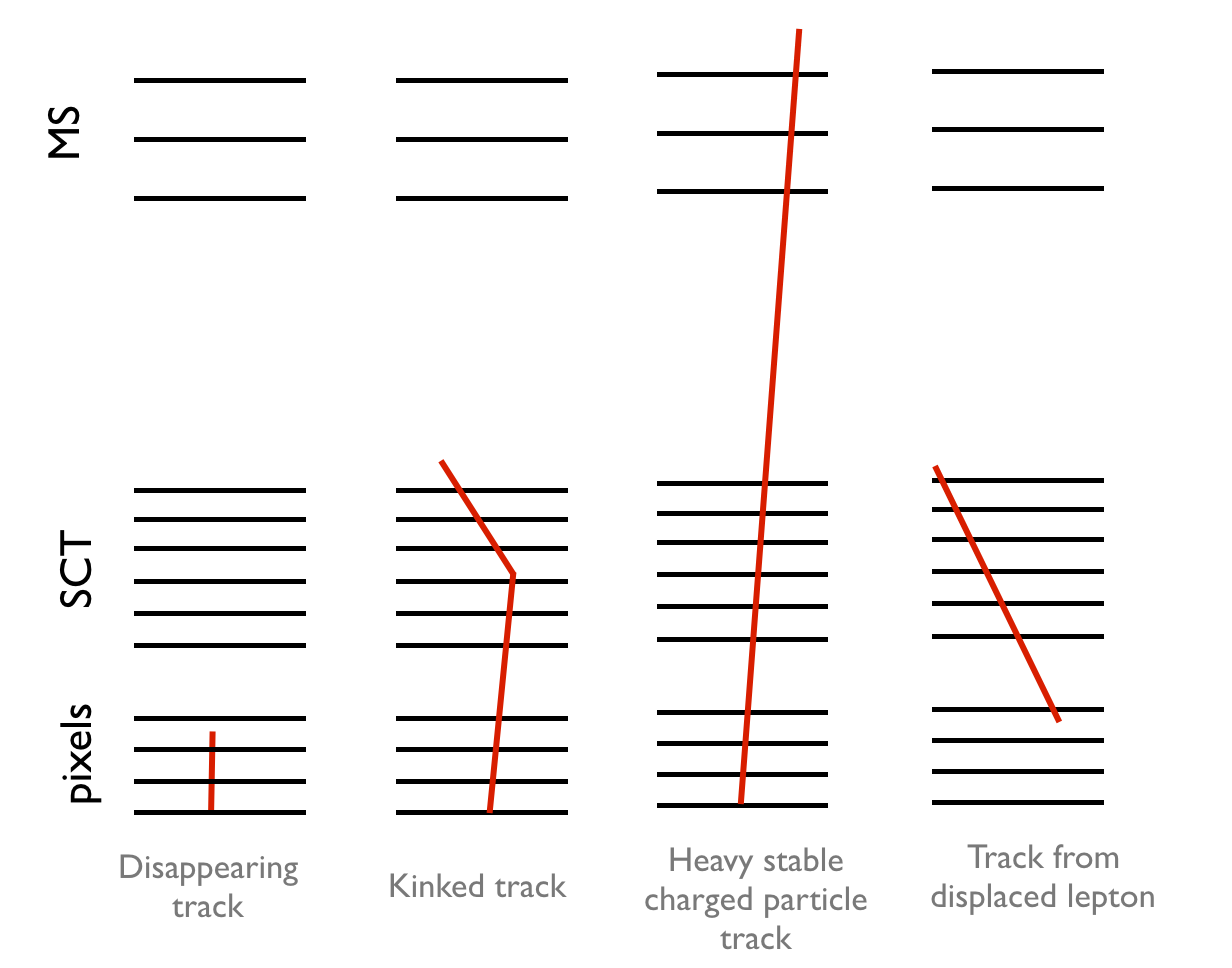
\includegraphics[width=.7\textwidth]{figures/theory/track-signatures.png}
\caption{A sketch of the various track signatures in a simplified \ac{ATLAS} detector that give sensitivity to displaced leptons. In reality, the tracks are curved by the magnetic fields in the \ac{ID} and \ac{MS}.}
\label{fig:track-sigs}
\end{figure}



\section{Previous Searches for Displaced Leptons}

The most stringent limits on long lived sleptons are the result of a searches from \ac{LEP} \cite{opal,L3,delphi,aleph,LEP-comb}. A search for different flavor ($e\mu$) displaced leptons was performed by \ac{CMS}, but did not target long lived sleptons and did not surpass the limit set at LEP \cite{cms-dl}. There are no \ac{ATLAS} searches that would select events with displaced leptons and no secondary vertex.

\subsection{LEP}
\label{sec:opal-limit}

The \ac{LEP} experiments searched for long-lived \slep signatures from the process $e^+e^-\rightarrow \slep^+_R \slep^-_R$. A combination of results from the LEP experiments (OPAL, L3, ALEPH, and DELPHI) excluded right-handed $\tilde{\mu}$ and $\tilde{e}$ of all lifetimes with masses less than 96.3 GeV and 65.8 GeV, respectively. The OPAL experiment alone set the best limits on all lifetimes of $\tilde{\tau}_1$, a mixture of left- and right-handed states, with masses less than 87.6 GeV. The OPAL search will be discussed in detail.

The OPAL experiment at \ac{LEP} set limits on long-lived \slep signatures and set limits on \slep lifetimes between $10^{-6}$ s (detector-stable) and $10^{-12}$ s (prompt signatures). The detector conditions of the $ee$ collider are much less busy than those of the $pp$ collider -- the extra particles and tracks created by low energy \ac{QCD} interactions between other partons in the proton or other protons in the bunch do not exist, simplifying the task of track reconstruction. The search was done with 600 pb$^{-1}$ of data with $\sqrt{s} = 189 - 209$ GeV between the years 1998 and 2000.

The portion of the analysis that targets displaced leptons has a relatively simple event selection. Events are required to have no prompt tracks and at least two tracks with opposite charges and $\dz > 5$ mm corresponding to the displaced leptons. To reduce backgrounds from cosmic-ray muons, a time-of-flight detector was used. To reduce beam-induced backgrounds, both tracks were required to have $\absz < 400$ mm. To reduce background from Bhahba scattering ($e^+e^- \rightarrow e^+e^-$ by exchanging a $\gamma$), the tracks were required to not be back-to-back. To reduce the background from di-photon events, tracks must have $pt > 10$ GeV and the invariant mass of the two tracks must be greater than 5 GeV. $0.13 \pm 0.76$ events were expected and zero were observed. To specifically probe the \stau decay, the track \pt and invariant mass requirements were loosened to 5 GeV and 3 GeV, respectively. Here, $3.79 \pm 1.71$ events were expected and 3 observed.

Additionally, this search targeted \slep with shorter lifetimes by looking for events with at least two leptons and \ac{MET}. Longer lifetimes were probed by looking for kinked tracks (see \autoref{fig:track-sigs}) where the tracks of the \slep and $\ell$ are both observed. Signatures of \slep with even longer lifetimes and escape the detector were targeted by looking for tracks with high ionization energy loss. No excess of events was observed in any of the signatures, and the limits set are shown in \autoref{fig:opal-limit}.


\begin{figure}[!h]
\centering
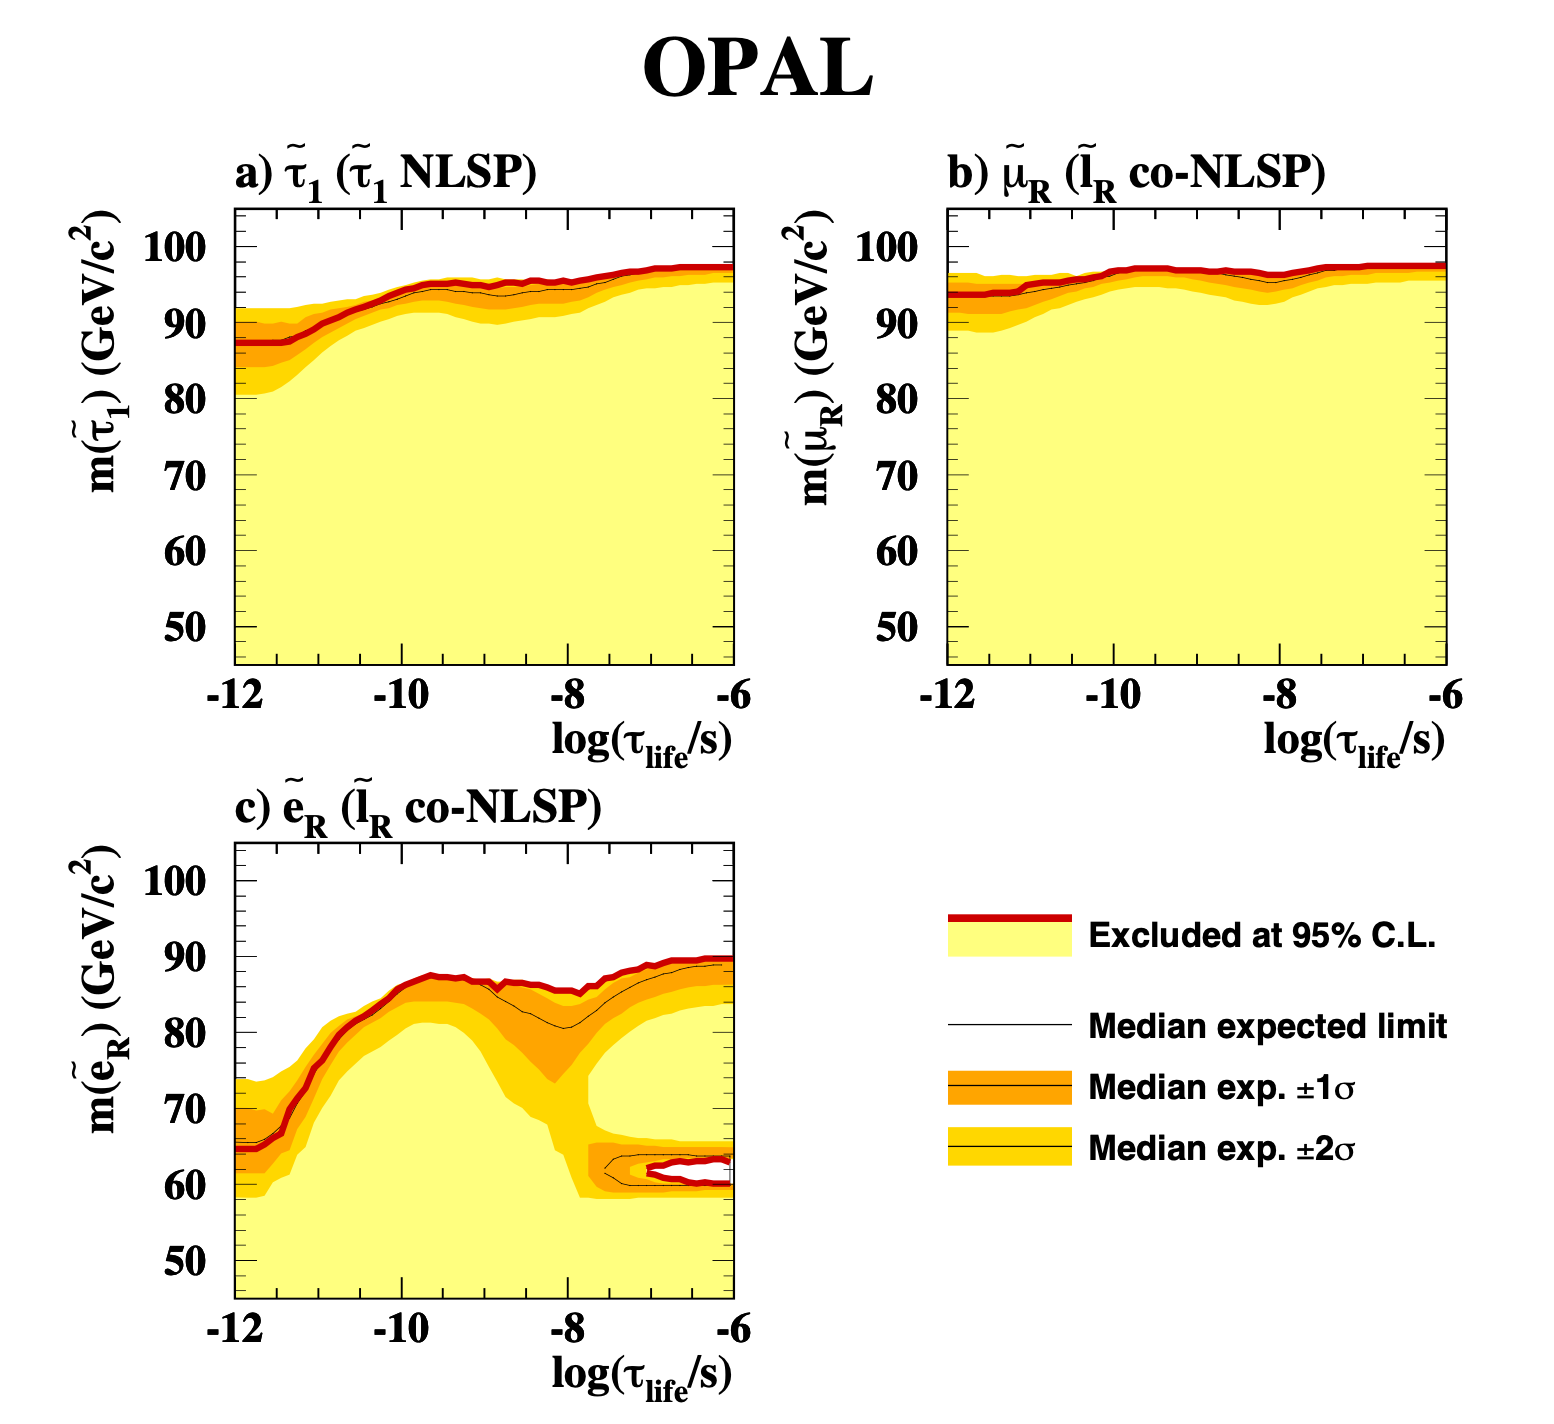
\includegraphics[width=.6\textwidth]{figures/theory/opal-limit.png}
\caption{Limits on \slep production set by the OPAL experiment for the \stau \ac{NLSP} scenario (top left) and \smu (top right) and \selec (bottom left) in the co-\ac{NLSP} scenario.~\cite{opal}}
\label{fig:opal-limit}
\end{figure}


\subsection{CMS}
\label{sec:cms-limit}

The only search for vertexless displaced leptons at the \ac{LHC} is from the \ac{CMS} experiment, and it did not target \slep decays. The target model used for this search is the RPV $\tilde{t}$ decay described in \autoref{sec:othermodels}. The search is for differently flavored leptons ($e\mu$) only. 2.6 \ifb of $\sqrt{s} = 13$ TeV data taken during 2015 was used.  

The events are collected using a trigger that selects events with an electron and a muon and are then categorized into three signal regions, defined by the \absdz of the leptons shown in \autoref{fig:cms-regions}. The leptons must have $\pt > 25$ GeV, $\absdz > 0.1$ mm, opposite electric charges, and be separated ($\dR > 0.4$). Dominant backgrounds are from decays of heavy flavor hadrons (like b-hadrons) due to the small impact parameter requirement (the search in this thesis requires $\absdz > 3$ mm and the OPAL result requires $\absdz > 5$ mm). The background is estimated by extrapolating the \absdz distribution of leptons inside of jets to the signal region selections. No excess was observed and a reinterpretation of this search \cite{jesseshelton} shows that this result does not exceed the limit from \ac{LEP}.


\begin{figure}[!h]
\centering
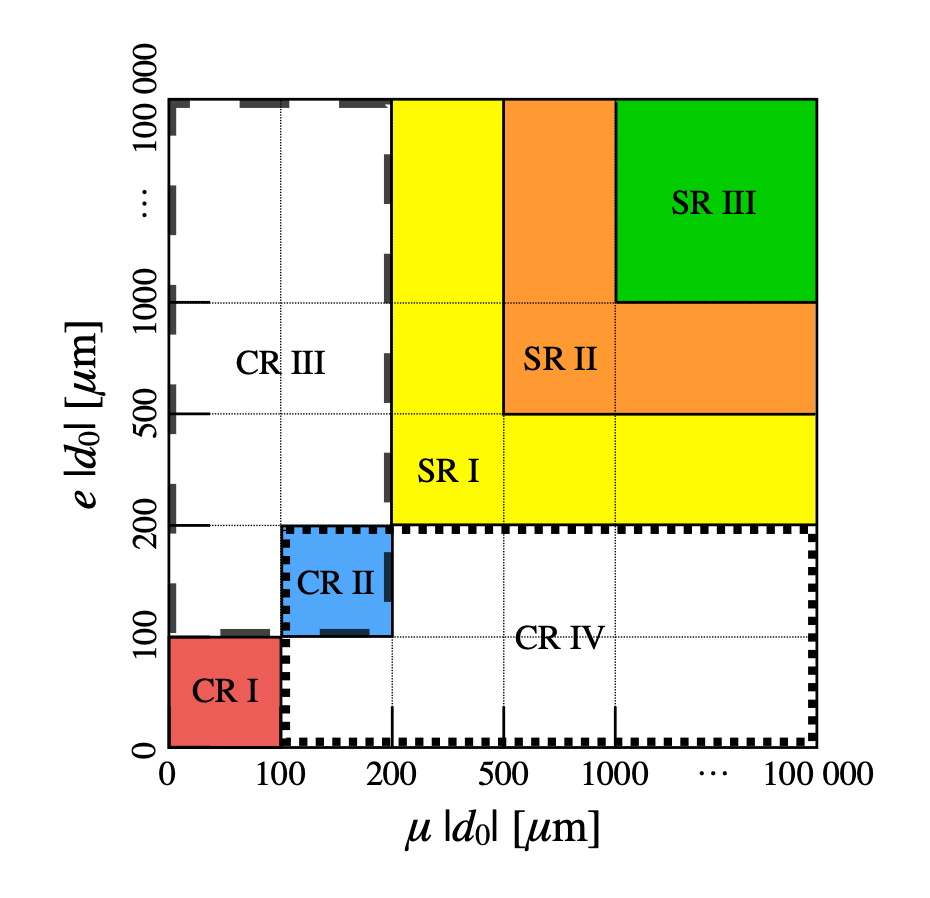
\includegraphics[width=.6\textwidth]{figures/theory/cms-dl.png}
\caption{Signal and control regions used by CMS in Ref.~\cite{cms-dl}. The signal regions have significantly lower \absdz ($> 0.2$ mm) than in this thesis search ($> 3$ mm).}
\label{fig:cms-regions}
\end{figure}


\section{Other Signatures with Sensitivity to Long Lived Sleptons}

There are no constraints on the possible lifetime of a \slep in a \ac{GMSB} model, so various searches must be done together to cover the whole phase space. The displaced lepton signature covers an intermediate lifetime range. Searches for longer lifetimes look directly for the signature of the \slep instead of its decay products. \slep that decay in the tracker are covered by disappearing track searches \cite{SUSY-2016-06,CMS-EXO-16-044,SUSY-2011-14,CMS-EXO-12-034} and those which are detector stable are probed by searches for tracks consistent with those from a heavy stable charged particle \cite{SUSY-2016-02,SUSY-2011-03,CMS-EXO-16-044}. These signatures have been covered by both \ac{ATLAS} and \ac{CMS}. While they did not directly target long lived \slep, the reinterpretation done by Ref. \cite{jesseshelton} shows that they improve significantly over the OPAL result. All constraints on \slep production as determined by Ref. \cite{jesseshelton} are shown in \autoref{fig:jesse}. 

\begin{figure}[!h]
\centering
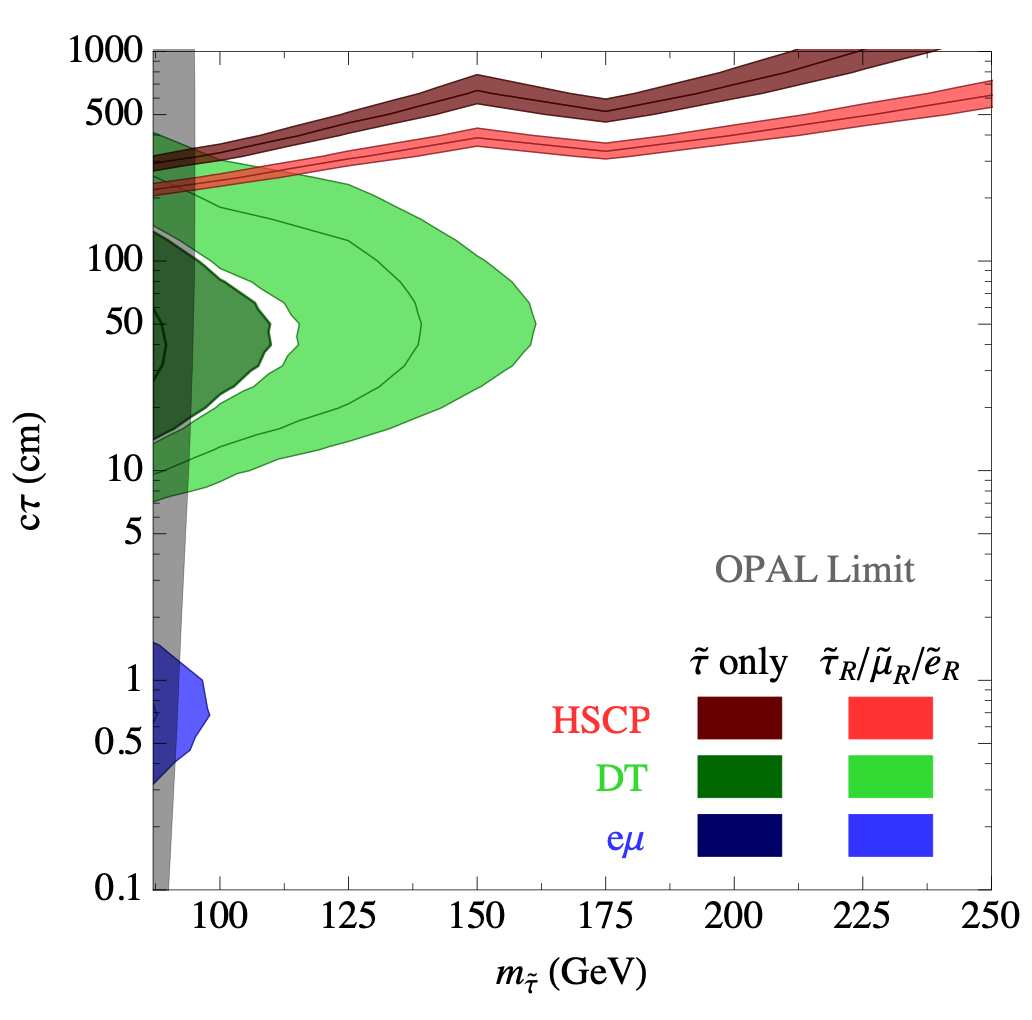
\includegraphics[width=.6\textwidth]{figures/theory/slep-limits.png}
\caption{Constraints on direct production of long lived \slep. \stau and co-NLSP scenarios are shown in darker and brighter colors, respectively. The OPAL result discussed in \autoref{sec:opal-limit} is shown in gray and \ac{CMS} result discussed in \autoref{sec:cms-limit} is shown in blue. Constraints from disappearing track signatures (DT) discussed in \autoref{sec:dt-limit} is shown in green, and constraints from heavy stable charged particle signatures (HSCP) discussed in \autoref{sec:hscp-limit} is shown in red. The \ac{LHC} searches are from Run 1, with $\sqrt{s} = 8$ TeV. The search in this thesis covers the $c \tau$ range 0.01--100 cm with masses up to 800 GeV for co-NLSP scenarios. \cite{jesseshelton}}
\label{fig:jesse}
\end{figure}


\subsection{Disappearing Tracks}
\label{sec:dt-limit}

A \emph{disappearing track} is a short track measured in the \acf{ID}. This track has hits in the innermost \ac{ID} layers and no hits along the rest of its trajectory In reality, the signature from a \slep decay is a kinked track, as targeted by OPAL. However, looking for kinked tracks is extremely difficult in the \ac{LHC} environment as kink be at any angle and any point along the track.

Both \ac{ATLAS} and \ac{CMS} look for a high \pt track with no hits in the outer layers of the tracking detector. These events are triggered based on their large \ac{MET} resulting from gravitino. Events are also required to have at least one high \pt jet ($\pt > 90$ GeV) with other jets well separated from each other and the \ac{MET}. They must also have no muon or electron candidates. This signature has sensitivity to \stau with hadronic $\tau$ decays.


\subsection{Heavy Stable Charged Particle Tracks}
\label{sec:hscp-limit}

Should a sufficiently heavy (detector-)stable charged particle be produced in \ac{LHC} collisions, it would pass through the entire detector leaving tracks in both the \ac{ID} and \ac{MS}. The signature is a track with an \ac{ID} tracks matched to \ac{MS} tracks. A time-of-flight measurement is made using the \ac{MS} and the \ac{MS} track must be consistent with a slow moving particle, as a heavy particle would likely have most of its energy in its mass and very low momentum. Ionization loss measurements in the Pixel detector can also be used to identify heavy, slow moving particles. The mean energy loss per unit space increases with the $\beta \gamma$ of a particle, as well as with it's mass according to the Bethe-Bloch formula~\cite{pdg}.


In conclusion, \slep with lifetimes between $10^{-11}$ ns and $10^{1}$ ns have much more unexplored phase space than other lifetime ranges. The vertex-less displaced di-lepton signature covers this region of parameter space. This thesis presents the first search to target this model at \ac{LHC} energies.
